\subsection{使用深度确定性策略梯度解决倒立摆问题}

前面章节都是离散动作的环境,但实际中也有很多连续动作的环境,比如 OpenAI Gym 中的 Pendulum-v1 环境,它解决的是一个倒立摆问题,我们先对该环境做一个简要说明。

\subsubsection{ Pendulum-v1 简介}

如果说 CartPole-v0 是一个离散动作的经典入门环境,那么 Pendulum-v1 就是连续动作的经典入门环境。如\figref{fig:pendulum_1} 所示,我们通过施加力矩使摆阵向上摆动并保持直立。

\begin{figure}[htb]
    \centering
    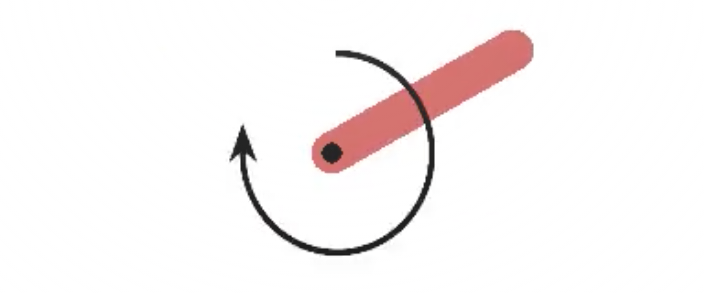
\includegraphics[width=0.3\linewidth]{res/ch12/assets/pendulum_1.png}
    \caption{Pendulum-v1环境}
    \label{fig:pendulum_1}
\end{figure}
该环境的状态数有三个,设摆针在竖直方向上的顺时针旋转角为$\theta$,$\theta$设在$[\mathrm{\pi},\mathrm{\pi}]$之间,则相应的状态为$[cos\theta,sin\theta,\dot{\theta}]$,即表示角度和角速度.我们的动作则是一个 $-2$ 到 $2$ 之间的力矩,它是一个连续量,因而该环境不能用离散动作的算法比如深度 Q 网络算法来解决。奖励是根据相关的物理原理而计算出的等式,如下:

$$
-\left(\theta^{2}+0.1 \times \hat{\theta}^{2}+0.001 \times \text { action }^{2}\right)
$$

对于每一步,其最低奖励为$-\left(\mathrm{\pi}^{2}+0.1 \times 8^{2}+0.001 \times 2^{2}\right)= -16.2736044$,最高奖励为0。同 CartPole-v0 环境一样,达到最优算法的情况下,每回合的步数是无限的,因此这里设定每回合最大步数为200以便于训练。

\subsubsection{ 深度确定性策略梯度基本接口}

我们依然使用接口的概念,通过伪代码分析并实现 DDPG 的训练模式,如\figref{fig:ddpg} 所示。

\begin{figure}[htb]
    \centering
    
\includegraphics[width=0.75\linewidth]{res/ch12/assets/ddpg.png}
    \caption{深度确定性策略梯度算法}
    \label{fig:ddpg}
\end{figure}

代码如下:

\begin{lstlisting}[style=Python]
    ou_noise = OUNoise(env.action_space)  # 动作噪声
    rewards = [] # 记录奖励
    ma_rewards = []  # 记录滑动平均奖励
    for i_ep in range(cfg.train_eps):
        state = env.reset()
        ou_noise.reset()
        done = False
        ep_reward = 0
        i_step = 0
        while not done:
            i_step += 1
            action = agent.choose_action(state)
            action = ou_noise.get_action(action, i_step) 
            next_state, reward, done, _ = env.step(action)
            ep_reward += reward
            agent.memory.push(state, action, reward, next_state, done)
            agent.update()
            state = next_state
        if (i_ep+1)%10 == 0:
            print('回合:{}/{},奖励:{}'.format(i_ep+1, cfg.train_eps, ep_reward))
        rewards.append(ep_reward)
        if ma_rewards:
            ma_rewards.append(0.9*ma_rewards[-1]+0.1*ep_reward)
        else:
            ma_rewards.append(ep_reward)
\end{lstlisting}

相比于 深度Q网络 , DDPG 主要更新了两部分,一是给动作施加噪声,另外是软更新策略,即最后一步。

\subsubsection{ Ornstein-Uhlenbeck 噪声}

奥恩斯坦-乌伦贝克(Ornstein-Uhlenbeck,OU)噪声适用于惯性系统,尤其是时间离散化粒度较小的情况。 OU 噪声是一种随机过程,下面略去证明,直接给出公式。对于当前时刻$t$的一个变量$x$,其下一时刻$x(t+\Delta t)$:
$$
x(t+\Delta t)=x(t)-\theta(x(t)-\mu) \Delta t+\sigma W_t
$$
其中 $W_t$ 属于正态分布,OU 噪声代码实现如下:

\begin{lstlisting}[style=Python]
    class OUNoise(object):
        '''Ornstein–Uhlenbeck噪声
        '''
        def __init__(self, action_space, mu=0.0, theta=0.15, max_sigma=0.3, min_sigma=0.3, decay_period=100000):
            self.mu           = mu # OU噪声的参数
            self.theta        = theta # OU噪声的参数
            self.sigma        = max_sigma # OU噪声的参数
            self.max_sigma    = max_sigma
            self.min_sigma    = min_sigma
            self.decay_period = decay_period
            self.action_dim   = action_space.shape[0]
            self.low          = action_space.low
            self.high         = action_space.high
            self.reset()
        def reset(self):
            self.obs = np.ones(self.action_dim) * self.mu
        def evolve_obs(self):
            x  = self.obs
            dx = self.theta * (self.mu - x) + self.sigma * np.random.randn(self.action_dim)
            self.obs = x + dx
            return self.obs
        def get_action(self, action, t=0):
            ou_obs = self.evolve_obs()
            self.sigma = self.max_sigma - (self.max_sigma - self.min_sigma) * min(1.0, t / self.decay_period) # sigma会逐渐衰减
            return np.clip(action + ou_obs, self.low, self.high) # 动作加上噪声后进行剪切
\end{lstlisting}

\subsubsection{深度确定性策略梯度算法}

 DDPG 算法主要也包括两个功能,一个是选择动作,另外一个是更新策略,首先看选择动作:

\begin{lstlisting}[style=Python]
    def choose_action(self, state):
        state = torch.FloatTensor(state).unsqueeze(0).to(self.device)
        action = self.actor(state)
        return action.detach().cpu().numpy()[0, 0]
\end{lstlisting}

由于 DDPG 是直接从演员网络取得动作,因此这里不用$\varepsilon$-贪心策略。在更新策略函数中,也会与 深度Q网络 稍有不同,并且加入软更新:

\begin{lstlisting}[style=Python]
    def update(self):
        if len(self.memory) < self.batch_size: # 当 memory 中不满足一个批量时,不更新策略
            return
        # 从回放缓冲区中随机采样一个批量的经验
        state, action, reward, next_state, done = self.memory.sample(self.batch_size)
        # 转变为张量
        state = torch.FloatTensor(state).to(self.device)
        next_state = torch.FloatTensor(next_state).to(self.device)
        action = torch.FloatTensor(action).to(self.device)
        reward = torch.FloatTensor(reward).unsqueeze(1).to(self.device)
        done = torch.FloatTensor(np.float32(done)).unsqueeze(1).to(self.device)
        # 计算期望Q值
        policy_loss = self.critic(state, self.actor(state))
        policy_loss = -policy_loss.mean()
        next_action = self.target_actor(next_state)
        target_value = self.target_critic(next_state, next_action.detach())
        expected_value = reward + (1.0 - done) * self.gamma * target_value
        expected_value = torch.clamp(expected_value, -np.inf, np.inf)
        value = self.critic(state, action)
        value_loss = nn.MSELoss()(value, expected_value.detach())
        self.actor_optimizer.zero_grad()
        policy_loss.backward()
        self.actor_optimizer.step()
        self.critic_optimizer.zero_grad()
        value_loss.backward()
        self.critic_optimizer.step()
        # 软更新
        for target_param, param in zip(self.target_critic.parameters(), self.critic.parameters()):
            target_param.data.copy_(target_param.data * (1.0 - self.soft_tau) +param.data * self.soft_tau)
        for target_param, param in zip(self.target_actor.parameters(), self.actor.parameters()):
            target_param.data.copy_(target_param.data * (1.0 - self.soft_tau) +param.data * self.soft_tau)
\end{lstlisting}

\subsubsection{结果分析}

实现算法之后,我们先看看训练效果,如\figref{fig:train_rewards_curve_cn-1760758} 所示。

\begin{figure}[htb]
    \centering
    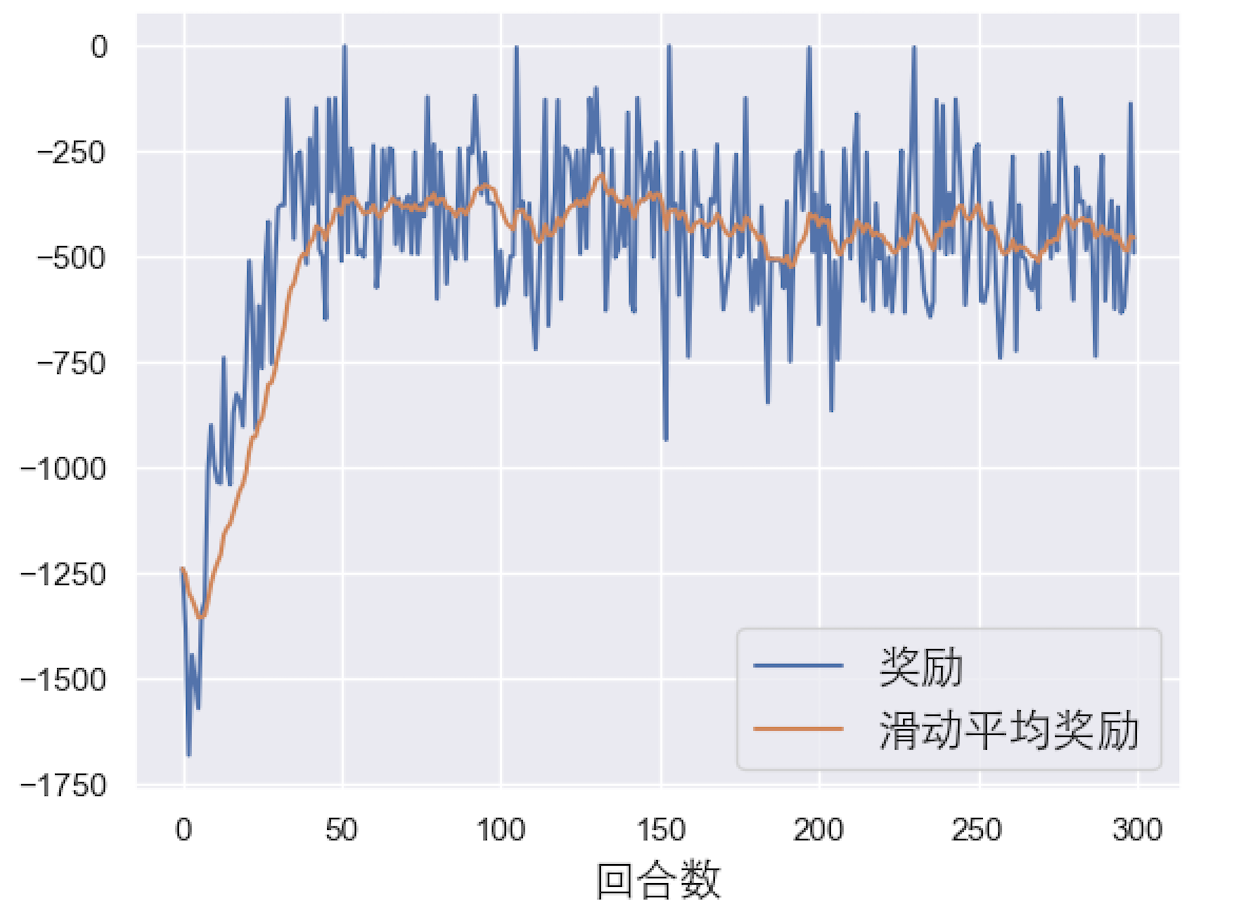
\includegraphics[width=0.6\linewidth]{res/ch12/assets/train_rewards_curve_cn-1760758.png}
    \caption{Pendulum-v1 环境下DDPG算法的训练曲线}
    \label{fig:train_rewards_curve_cn-1760758}
\end{figure}


可以看到算法整体上是收敛的,但是稳定状态下波动还比较大,依然有提升的空间。限于笔者的精力,这里只是帮助读者实现一个基础的代码演示,想要使得算法调到最优,感兴趣的读者可以多思考实现。我们再来看看测试的结果,如\figref{fig:eval_rewards_curve_cn-1760950} 所示。

\begin{figure}[htb]
    \centering
    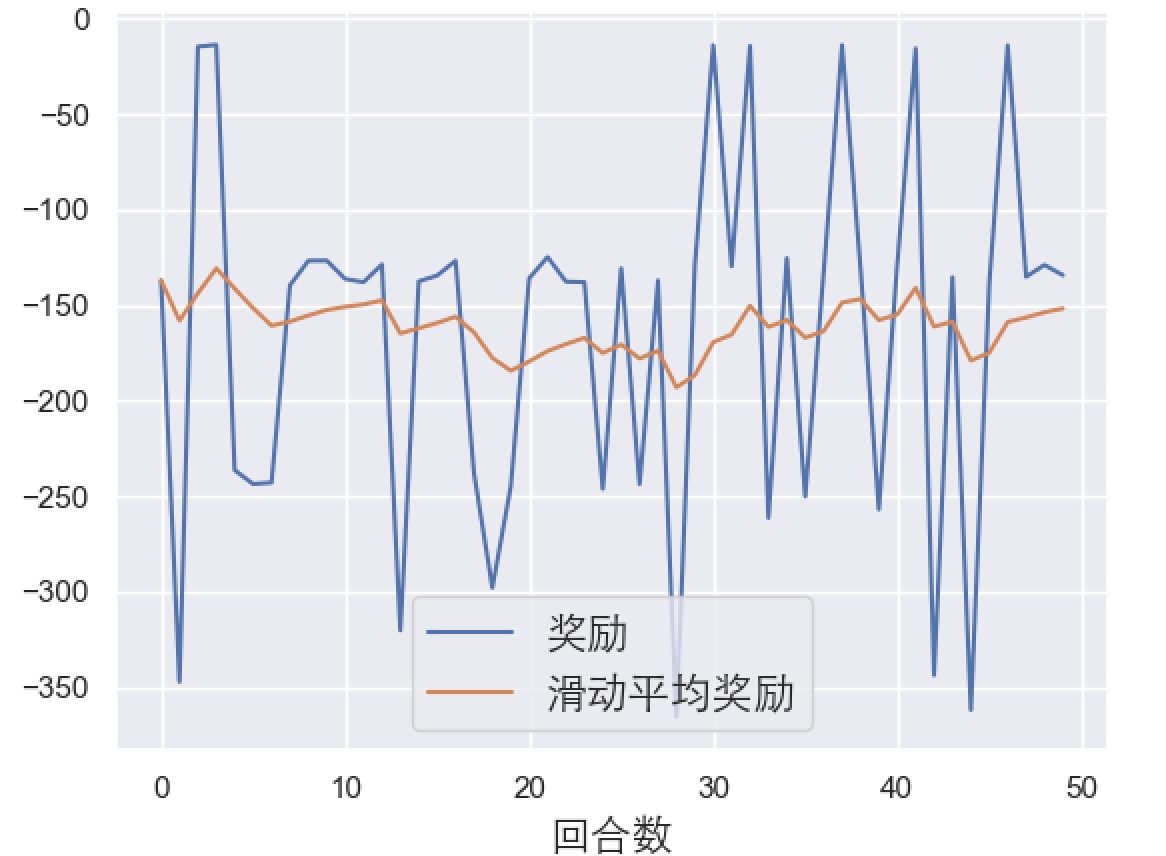
\includegraphics[width=0.6\linewidth]{res/ch12/assets/eval_rewards_curve_cn-1760950.png}
    \caption{Pendulum-v1 环境下DDPG算法的测试曲线}
    \label{fig:eval_rewards_curve_cn-1760950}
\end{figure}

从\figref{fig:eval_rewards_curve_cn-1760950} 中看出测试的滑动平均奖励在$-150$左右,但其实训练的时候平均的稳态奖励在$-300$左右,这是因为在测试的时候我们舍去了 OU 噪声。
